% Math symbols and examples: http://en.wikibooks.org/wiki/LaTeX/Mathematics
% Also useful link: http://en.wikibooks.org/wiki/LaTeX/Advanced_Mathematics

% This document is used for title generating of exercise solutions. 
% Also it used for generating styles and environmentof documents.
% To add this title in document add next line:
% % This document is used for title generating of exercise solutions. 
% Also it used for generating styles and environmentof documents.
% To add this title in document add next line:
% % This document is used for title generating of exercise solutions. 
% Also it used for generating styles and environmentof documents.
% To add this title in document add next line:
% \input{../template.tex}
\documentclass[a4paper]{article}
\usepackage[utf8]{inputenc}
\usepackage[top=1.5cm]{geometry}
\usepackage{amssymb}
\usepackage{enumitem}
\usepackage{amsmath}

\allowdisplaybreaks

\DeclareMathOperator{\ggT}{ggT}
\DeclareMathOperator{\kgV}{kgV}

\title{Mathematik: Diskrete Strukturen \\ \Large Lösungsblatt}
\author{Anton Bubnov, Eugen Kuzmenko}

\documentclass[a4paper]{article}
\usepackage[utf8]{inputenc}
\usepackage[top=1.5cm]{geometry}
\usepackage{amssymb}
\usepackage{enumitem}
\usepackage{amsmath}

\allowdisplaybreaks

\DeclareMathOperator{\ggT}{ggT}
\DeclareMathOperator{\kgV}{kgV}

\title{Mathematik: Diskrete Strukturen \\ \Large Lösungsblatt}
\author{Anton Bubnov, Eugen Kuzmenko}

\documentclass[a4paper]{article}
\usepackage[utf8]{inputenc}
\usepackage[top=1.5cm]{geometry}
\usepackage{amssymb}
\usepackage{enumitem}
\usepackage{amsmath}

\allowdisplaybreaks

\DeclareMathOperator{\ggT}{ggT}
\DeclareMathOperator{\kgV}{kgV}

\title{Mathematik: Diskrete Strukturen \\ \Large Lösungsblatt}
\author{Anton Bubnov, Eugen Kuzmenko}

\usepackage{wrapfig}
\begin{document}
    \maketitle
    \section*{Vertiefung:}
    \begin{enumerate}[label=(\alph*)]
        % Task (a)
        \item  Ein ebener,
        k-regulärer Graph besteht aus
        12 Knoten und teilt die Ebene in
        14 Gebiete. Wie groß ist k? \\
        Nach Theorem 3.23 gilt $||F|| = ||E|| - ||V|| + 2$. Für unseren Fall bedeutet das also:
        $14 = ||E|| - 12 + 2 \implies E = 24$ \\
        Des weiteren gilt nach Proposition 3.3: \\
        $\sum_{v \in V} deg(v) = 2 \cdot ||E||$. D.h. die Summe der Grade ist $2 * 24 = 58$. \\
        Daraus folgt $\frac{58}{12} = 4 = k$
        
        %Task (b)
        \item Aus Theorem 3.23 folgt, dass $||F|| = ||E|| - ||V|| + 2 gilt $. Für unseren Fall bedeutet 
        das aus $ 14 = ||E|| - 8 + 2 $ $ ||E|| = 20 $ folgt. Wir haben also einen Graphen mit 8 Knoten 
        und 20 Kanten. Nach Theorem 3.24 gilt für jeden planaren Graphen $ ||E|| \leq 3 \cdot ||V|| - 6$. 
        Für unseren Fall gilt also $20 \leq 3 \cdot 8 - 6  = 18$.
        Wir stoßen auf einen Widerspruch, da $20 \leq 18$ falsch ist. Einen solchen Graphen kann es nicht geben.
        
        %Task (c)
        \item Für einen planaren nicht-zusammenhängenden Graphen G mit k Zusammenhangskomponenten beachten 
        wir, dass sich die Komponenten die äußere Fläche gemeinsam teilen. Daraus folgt, dass es im gegensatz 
        zum zusammenhängenden Fall k-1 Flächen weniger gibt. Somit gilt für nicht zusammenhängende Graphen 
        $||F|| = ||E|| - ||V|| + 2 + (k-1) = ||E|| - ||V|| + 1 + k$. Für nicht-zusammenhängende Graphen 
        ergibt sich folglich: $||F|| = ||E|| - ||V|| + 1 + k $
       
        %Task (d)
        \item Ist der $Q_3$ planar? 
        Ja. Betrachte dazu folgende Graphik:\\
        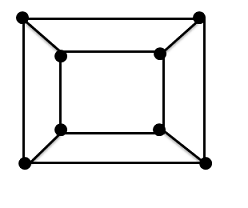
\includegraphics{Q3}
        
        %Task (e)
        \item Ist der $Q_4$ planar?
        Nein. Der $Q_4$ enthält einen $K_{3,3}$ als Teilgraphen. wenn man diesen Teilgraphen "aufspannt" 
        gibt es Überkreuzungen im gesamten Graphen. Daraus folgt, dass der $Q_4$ nicht planar sein kann.
        
        %Task (f)
        \item Es reicht aus die Aussage für kantenmaximale planare Graphen zu zeigen, da hiermit die 
        linke Seite maximiert wird. Sei nun $G=(V,E)$ ein kantenmaximaler und ebener Graph, der keine 
        Dreiecke als Teilgraphen besitzt. Für $||V||=3$ gibt es nur das Äußere und somit nur ein Gebiet. 
        Wenn wir nun einen Knoten hinzufügen, dann müssen wir auch aufgrund der Kantenmaximalität zwei 
        Kanten hinzufügen, wodurch Dreiecke vermieden werden.  Wenn wir dies fortsetzen, erhalten wir: \\ 
        $ 2 \cdot ||F|| \le ||E||\implies 2 \cdot \left(||E|| - ||V|| + 2 \right) \le ||E||$ \\ 
        Nach Theorem 3.23 gilt somit:
        $||E|| \le 2 \cdot ||V|| - 4 $. 
        
        % Task (g)
        \item
        
        % Task (h)
        \item

        % Task (i)
        \item Wie viele Knotenfärbungen mit k Farben hat ein $K_n$ ?
        Da jeder Knoten n-1 Nachbarn hat (jeder Knoten ist mit jedem verbunden) hat der $K_n$ $n$ Farben. 
        Der erste Knoten kann beliebig gewählt werden, weshalb es $k$ Möglichkeiten zur Färbung gibt. 
        Für die weiteren Knoten gibt es immer eine Möglichkeit weniger, für eine Färbung. Folglich gibt es: \\
        $\prod_{i=0}^{k-1} k - i$ Möglichkeiten zur Färbung eines $K_n$
          
        % Task (j)
        \item
        
    \end{enumerate}
    \section*{Kreativität:} Wie viele Knotenfärbungen mit 3 Farben hat der Kreis $C_n$ ?\\
        Hinweis: Stellen Sie eine geeignete Rekursionsgleichung auf und lösen Sie diese.\\\\
        Wenn wir anfangen die Knotenfärbungen sehen wir, dass beim jeder Kanten haben wir mehere 
        Möglichkeiten eine Farbe zu wählen. Da stellen wir diese Möglichkeiten als ein Baum vor. 
        Dann bekommen wir ein Beispiel mit der Farben $(1,2,3)$ und erste Knoten als 1 bewertet:
        \begin{wrapfigure}{l}{0.25\textwidth}
            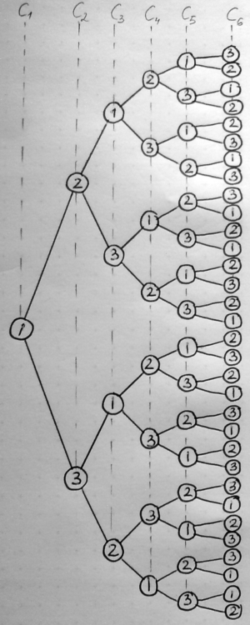
\includegraphics[width=1\linewidth]{baum_kreativ}
        \end{wrapfigure}\\
        Dann wir können sehen, alle Variationen für Kreis Länge $C_1$ bis $C_6$ und unseres Baum ein 
        Binärbaum ist. Da müssen wir aber beachten, dass manche Knoten passen uns nicht, und zwar die, 
        die Farbe 1 haben. Sehen wie der Kreis Länge 6 ein. Da sehen wir, dass die gesamte Anzahl der 
        Knoten $2^n-1$ ist, wo $n$ ist Länge der Kreis. Von 32 Knoten uns passen nur solche, die nicht 
        gleich 1 sind, also nur 22. Ferner merken wir, dass die Anzahl der 1 ist gleich wie die Anzahl 
        der passende Kanten aus $C_5$, weil die nur aus 2 oder 3 kommt und nur einmal pro jede Knote. 
        Da dieser Beispiel ist nur für 1 und wir drei Farben haben, sollen wir unsere Kombinationen 
        mit drei multiplizieren. Dann schreiben wir ein rekursiver Formel, der Knotenfärbungen Anzahl 
        berechnet, und zwar: $$ a_n = 3\cdot 2^{n-1} - a_{n-1} $$
        Jetzt sollen wir ein nicht-rekursive Formel finden. Schreiben wir erste 5 Knotenfärbungen:
        \begin{align*}
            a_0 &= 0\\
            a_1 &= 0\\
            a_2 &= 3\cdot 2^1 - a_1 = 3\cdot 2^1\\
            a_3 &= 3\cdot 2^2 - a_2 = 3\cdot 2^2 - 3\cdot 2^1\\
            a_4 &= 3\cdot 2^3 - a_3 = 3\cdot 2^3 - (3\cdot 2^2 - 3\cdot 2^1)\\
            a_5 &= 3\cdot 2^4 - a_4 = 3\cdot 2^4 - (3\cdot 2^3 - (3\cdot 2^2 - 3\cdot 2^1))\\
            &= 3\cdot 2^4 - 3\cdot 2^3 + 3\cdot 2^2 - 3\cdot 2^1\\
            &= 3\cdot (2^4 - 2^3 + 2^2 - 2^1)
        \end{align*} 
        Dann es ist schon deutlich, dass wir rekursive Formel so überschreiben können:
        $$ a_n = 3 \cdot (-1)^{n-1} \cdot \sum_{n=1}^{n-1}(-2)^n$$
    \section*{Transfer:}
    \begin{enumerate}[label=(\alph*)]
    	\item Task a
    \end{enumerate}
\end{document}